\section{Versuchsdurchführung}

Die Durchführung findet im oben beschriebenen Versuchsaufbau statt.
Das Schaltkreisbild sieht ist dargestellt wie in Abbildung \ref{Abbildung7}.
Hierbei wird ein Signal von dem Frequenzgenerator in die RLC-Schaltung geschickt welches dann in dem Oszilloskop sichtbar gemacht wird.
Alle Werteinstellungen die hier relevant sind, werden angegeben im nachfolgenden aufgezählt: 


\begin{figure}[H]
    \centering
    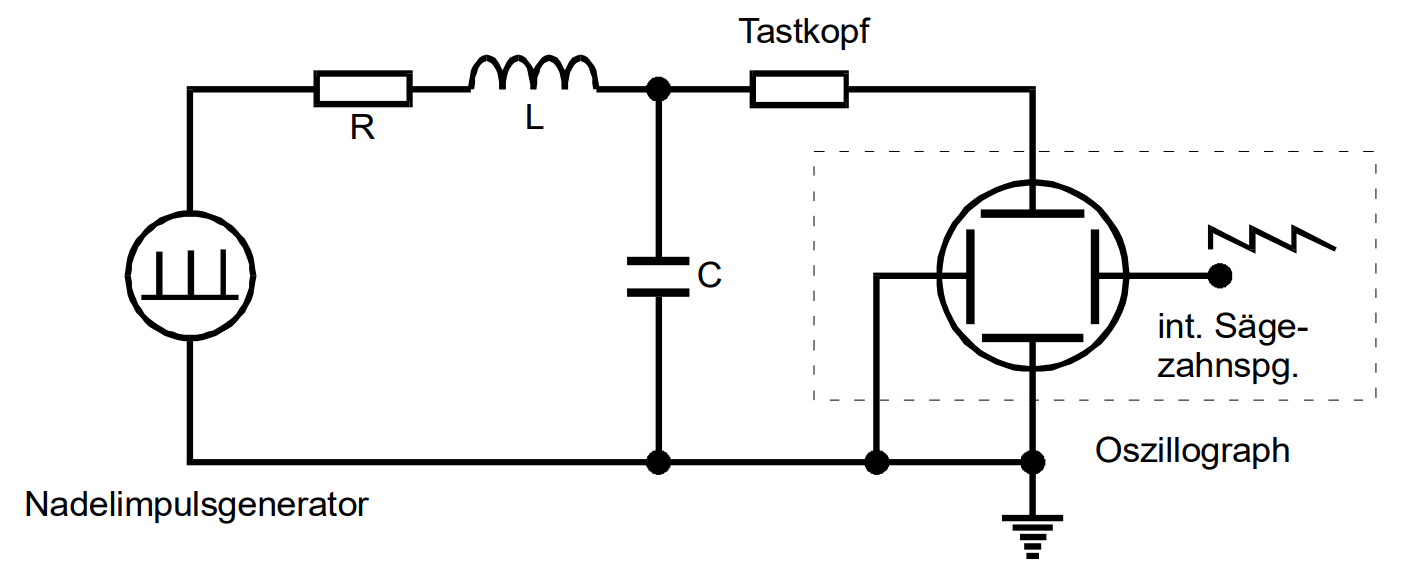
\includegraphics[width=90mm]{bilder/Ab6.png}
    \caption{Der Schaltkreisbild für Aufgabe 1 \cite[11]{GedUErzSch}. \label{Abbildung6}}
\end{figure}
 

\begin{flushleft}
    Im nächsten Arbeitsauftrag muss man mit dem Versuchsaufbau des vorherigen Arbeitsauftrages den Regler des variablen Widerstandes so einstellen,
    dass sich keine Wellen mehr \enquote{Überschwingen}. \\
\end{flushleft}


\begin{figure}[H]
    \centering
    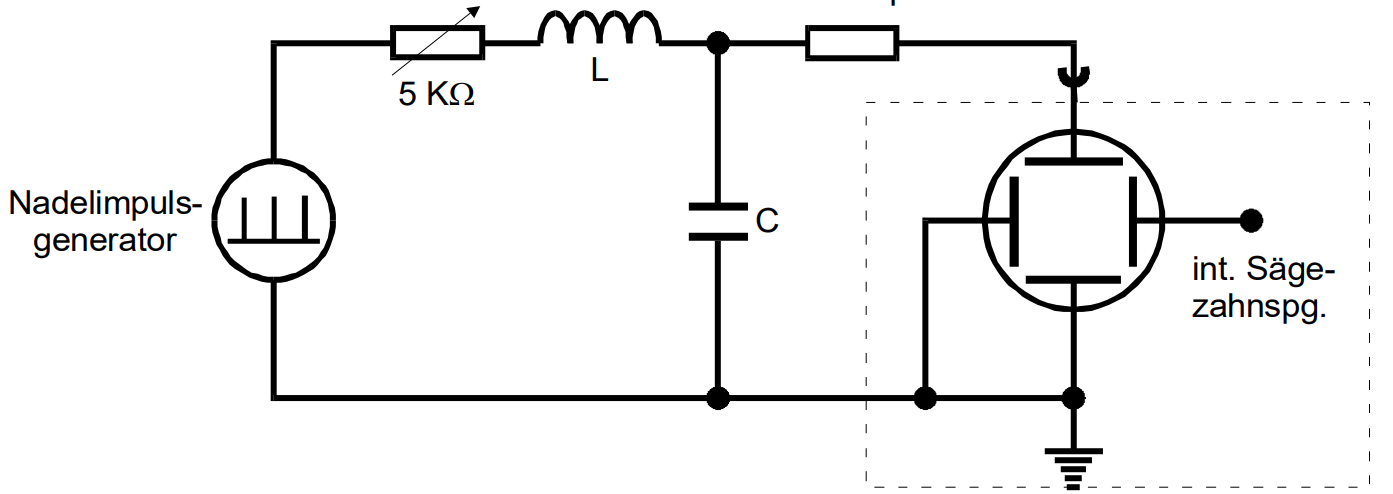
\includegraphics[width=90mm]{bilder/Ab7.png}
    \caption{Schaltkreisbild für Aufgabe 2 \cite[12]{GedUErzSch}. \label{Abbildung7}}
\end{figure}


\begin{figure}[H]
    \centering
    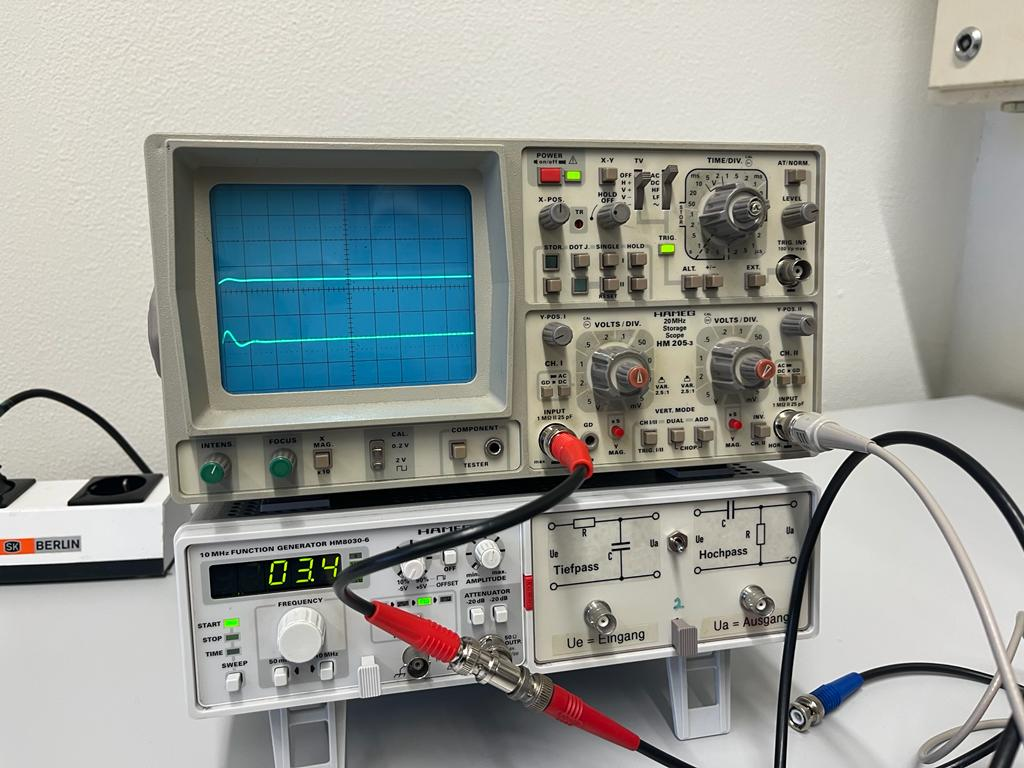
\includegraphics[width=90mm]{bilder/Ab8.jpeg}
    \caption{der Dämpfungswiderstand $\text{R}_\text{ap}$ verbildlicht. \label{Abbildung8}}
\end{figure}


\begin{flushleft}
    Als nächstes wird dem Versuchsaufbau ein Kabel hinzugefügt, welches 
    direkt von dem Generator zu dem Oszilloskop geht ohne durch die Schaltung zu gehen. \\
    Die Spannung die dabei gemessen wird ist $\text{U}_{0}$, wie in den Abbildung \ref{Abbildung9} und \ref{Abbildung5}.
\end{flushleft}


\begin{figure}[H]
    \centering
    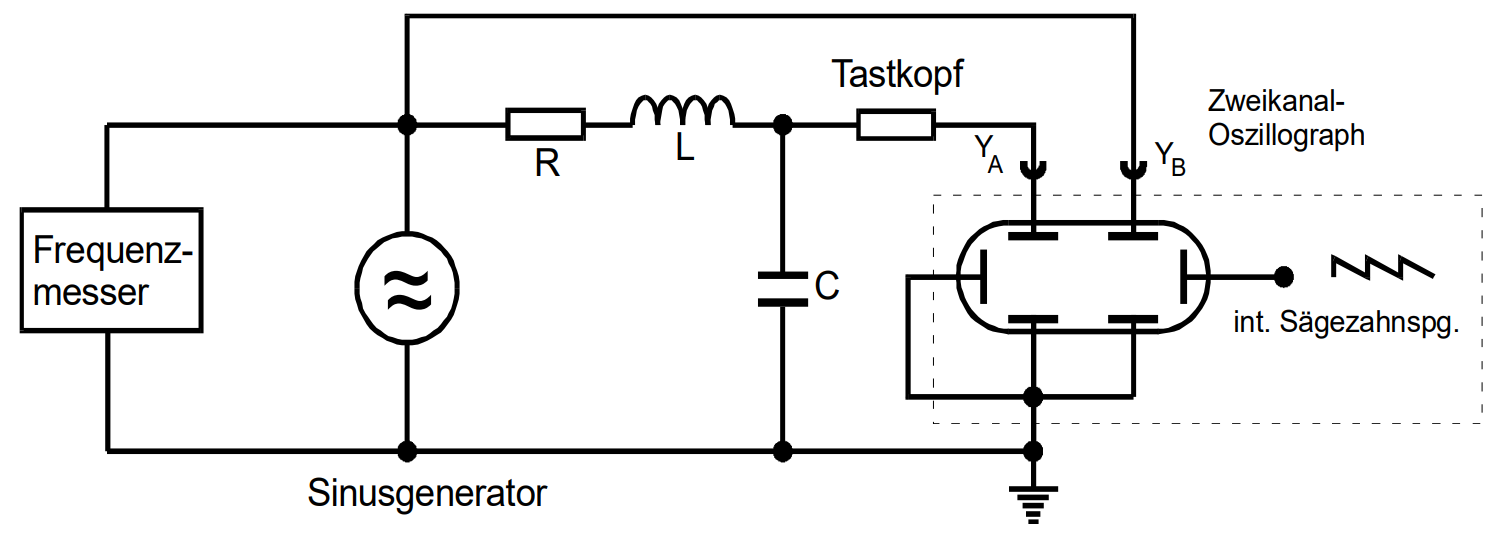
\includegraphics[width=90mm]{bilder/Ab9.png}
    \caption{Das Schaltkreisbild für Aufgabe 3 \cite[13]{GedUErzSch}. \label{Abbildung9}}
\end{figure}


\begin{flushleft}
    Als letztes wird der Versuchsaufbau des letzten Arbeitsauftrages verwendet und durch umstellen der Frequenz, die Phasenunterschiede 
    immer mehr sichtbar und größer gemacht.
\end{flushleft}
